\documentclass{article}

\usepackage[a4paper,top=1cm,bottom=1cm,left=1cm,right=1cm]{geometry}
\pagenumbering{gobble}
\setlength{\parindent}{0pt}
\usepackage{tgadventor}
\renewcommand*\familydefault{\sfdefault}
\usepackage[T1]{fontenc}
\usepackage{ragged2e}
\usepackage{graphicx} 
\usepackage{float}
\usepackage{wrapfig}
\usepackage{fontawesome5}
\usepackage{tikz}
\usepackage{tikzsymbols}
\usetikzlibrary{positioning}
\usepackage{pgffor}

\title{\Huge Escursione: <nome escursione>}
\date{}
\author{}

\begin{document}
\newcommand{\stanchezza}[2]{
\begin{tikzpicture}
    \node () at (-2,0) {LIVELLO DI STANCHEZZA};
    \foreach \i in {1,...,#1}{
    \node (\i) at (\i,0) {\Large\faBatteryFull}; }
    \ifnum #2>#1
        \foreach \i in {#1+1,...,#2}{
        \node (\i) at (\i,0) {\Large\faBatteryEmpty}; 
        }
    \fi
\end{tikzpicture}    
}

\newcommand{\esperienza}[2]{
\begin{tikzpicture}
    \node () at (-2,0) {VALUTAZIONE ESPERIENZA};
    \foreach \i in {1,...,#1}{
    \node (\i) at (\i,0) {\Large\faGrinStars}; }

    \ifnum #2>#1
        \foreach \i in {#1+1,...,#2}{
        \node (\i) at (\i,0) {\Large\faGrinStars[regular]};
        }
    \fi
        
\end{tikzpicture}    
}
\begin{tikzpicture}[main/.style = {draw, rectangle, rounded corners=0.1cm,minimum height = 0.5cm, minimum width=0.5cm}, align=center]
%\faTimes per inserire la crocetta :)
    \node [main] (t) {};
    \node (t1)[right=0.1 of t]{T};
    
    \node [main] (e) [right=0.4 of sun1] {};
    \node (e1)[right=0.1 of e]{E};
    
    \node [main] (ee) [right=0.4 of e1] {};
    \node (ee1)[right=0.1 of ee]{EE};
    
    \node [main] (eea) [right=0.4 of ee1] {\faTimes};
    \node (eea1)[right=0.1 of eea]{EEA};

    \node [main] (eai) [right=0.4 of eea1] {};
    \node (eai1)[right=0.1 of eai]{EAI};

\end{tikzpicture}
 \begin{tikzpicture}[main/.style = {draw, rectangle, rounded corners=0.1cm,minimum height = 0.5cm, minimum width=0.5cm}, align=center]
%\faTimes per inserire la crocetta :)
    \node [main] (sun) {}; 
    \node (sun1)[right=0.1 of sun]{\Large\faSun};
    
    \node [main] (cloudSun) [right=0.4 of sun1] {\faTimes};
    \node (cloudSun1)[right=0.1 of cloudSun]{\Large\faCloudSun};
    
    \node [main] (cloudSunRain) [right=0.4 of cloudSun1] {};
    \node (cloudSunRain1)[right=0.1 of cloudSunRain]{\Large\faCloudSunRain};
    
     \node [main] (shower) [right=0.4 of cloudSunRain1] {};
    \node (shower1)[right=0.1 of shower]{\Large\faCloudShowersHeavy};

    \node [main] (snow) [right=0.4 of shower1] {};
    \node (snow1)[right=0.1 of snow]{\Large\faSnowflake};
    

\end{tikzpicture}
\newcommand{\tipopercorso}[1]{
    \def\macroin{#1}
    \def\macroA{A}
    \def\macroAR{AR}
    \def\macroAnello{Anello}
    \begin{tikzpicture}[main/.style = {draw, rectangle, rounded corners=0.1cm,minimum height = 0.5cm, minimum width=0.5cm}, align=center]
    %\faTimes per inserire la crocetta :)
        \ifx\macroA\macroin
            \node [main] (a) {\faTimes};
            \node (a1)[right=0.1 of a]{$\longrightarrow$\\Solo Andata};    
        \else
            \node [main] (a) {};
            \node (a1)[right=0.1 of a]{$\longrightarrow$\\Solo Andata};
        \fi

        \ifx\macroR\macroin
            \node [main] (ar) [right=0.4 of a1] {\faTimes};
            \node (ar1)[right=0.1 of ar][minimum size = 0.01cm]{$\longrightarrow$\\
        $\longleftarrow$\\Andata e \\ritorno};  
        \else
            \node [main] (ar) [right=0.4 of a1] {};
            \node (ar1)[right=0.1 of ar][minimum size = 0.01cm]{$\longrightarrow$\\
        $\longleftarrow$\\Andata e \\ritorno};
        \fi

        \ifx\macroAnello\macroin
            \node [main] (anello) [right=0.4 of ar1] {\faTimes};
            \node (anello1)[right=0.1 of anello]{$\bigcirc$\\Ad anello};
        \else
            \node [main] (anello) [right=0.4 of ar1] {};
            \node (anello1)[right=0.1 of anello]{$\bigcirc$\\Ad anello};
        \fi

    \end{tikzpicture}
}
\maketitle

\begin{minipage}[t]{0.5\textwidth}
    \faCalendar* DATA:\\
    \\
    \faSmile[regular] COMPAGNIA:\\
    \\
    \faMapPin[regular] LUOGO DI PARTENZA:\\
    %Ora/Temperatura/Quota\\
    \\
    \faMapPin[regular] LUOGO DI ARRIVO:\\
    %Ora/Temperatura/Quota\\
    \\
    \faMountain[regular] CIME RAGGIUNTE:\\
    %\\
    \vspace*{1cm}\\
    KM PERCORSI:\\
    DISLIVELLO:\\
    DURATA:\\
    QUOTA MASSIMA:\\
\end{minipage} 
%NON INIZIARE NUOVO PARAGRAFO
\begin{minipage}[t]{0.4\textwidth}
    METEO: \\ \\
    \meteo{S}

    TIPO DI PERCORSO: \\ \\
    \tipopercorso{Anello}

    LIVELLO DI DIFFICOLT\'A: \\ \\
    \difficolta{T}

\end{minipage}
\centering

\raisebox{-7ex}{
    \begin{minipage}[H]{0.5\textwidth} %non riesco a togliere gli errori qui :(
        \stanchezza{2}{5}\\ %es: livello di stanchezza 2 su 5
        \\
        \esperienza{3}{5}  %es: valutazione generale 3 su 5
    \end{minipage}
}
\vspace*{1cm}\\
%tutte le foto che vuoiii <3
%\includegraphics[width=0.3\textwidth]{}
%\hspace{0.5cm}
%\includegraphics[width=0.3\textwidth]{}
%\hspace{0.5cm}
%\includegraphics[width=0.3\textwidth]{}

\vspace*{1cm}
NOTE: 

\end{document}
